\subsection{Interrelación Plantilla Entrevista Oficial - Pregunta Oficial}

   \begin{description}
      \item[Definición] En esta interrelación se deja constancia de que una
      plantilla de entrevista oficial puede estar compuesta por varias preguntas
      oficiales.

      \item[Características] La interrelación presenta las siguientes
                             características:

         \begin{itemize}
            \item \textbf{Nombre:} PEO-PO
            \item \textbf{Tipo de la interrelación:} El tipo de entidad Pregunta
                  Oficial es débil por identificación respecto al tipo de
                  entidad Plantilla Entrevista Oficial.
            \item \textbf{Cardinalidad de la interrelación:} 1:N
                  \begin{itemize}
                     \item Plantilla Entrevista Oficial: contiene (0,n)
                     \item Pregunta Oficial: forma\_parte\_de (1,1)
                  \end{itemize}
            \item \textbf{Número de atributos:} Ninguno.
         \end{itemize}

      \item[Diagrama] La figura \ref{diagramaPEO-PO} muestra el diagrama de la
                      interrelación.

      \item \begin{figure}[!ht]
            \begin{center}
            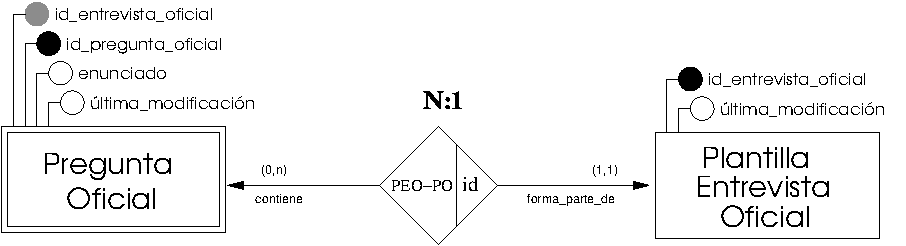
\includegraphics[]{07.Modelo_Entidad-Interrelacion/7.3.Analisis_Interrelaciones/diagramas/PEO-PO.pdf}
            \caption{Diagrama de la interrelación PEO-PO.}
            \label{diagramaPEO-PO}
            \end{center}
         \end{figure}

      \item[Ejemplo práctico del tipo de interrelación]

      \item \begin{center}
            \begin{tabular}{ | r r | }
            \hline
            \multicolumn{2}{ | c | }{\textbf{Tipo de interrelación PEO-PO}} \\
            \hline
            \textbf{Plantilla Entrevista Oficial} & \\
            id\_entrevista\_oficial & 24 \\
            \hline
            \textbf{Pregunta Oficial} & \\
            id\_entrevista\_oficial & 24 \\
            id\_pregunta\_oficial & 55 \\
            enunciado & ¿Quién le ha informado de esta carrera? \\
            \hline
            \end{tabular}
         \end{center}
   \end{description}
